\section{SIMD nodes}

\ac{SIMD} nodes are the main processing elements of the image processor and are
responsible for carrying out image processing instructions in parallel. They
share the same instruction set and executes them in parallel, hence
\acf{SIMD}.

Each \ac{SIMD} node is fully equipped with a register bank,
an \ac{ALU} and data exchange with adjacent nodes.
Everything inside the node is operated through the SIMD node
instruction set explained in \ref{subsection:}.

The schematic of a single \ac{SIMD} node is shown in Figure
\ref{fig:fpga-simd-arch}, and details the entire data-path for the
node. External inputs to the node are drawn on the left side. Data-buses are 
marked as blue lines while control signals are red dashed lines. In the 
following section we will refer to this image when explaining the different 
components.

\begin{figure}[h]
  \centering
 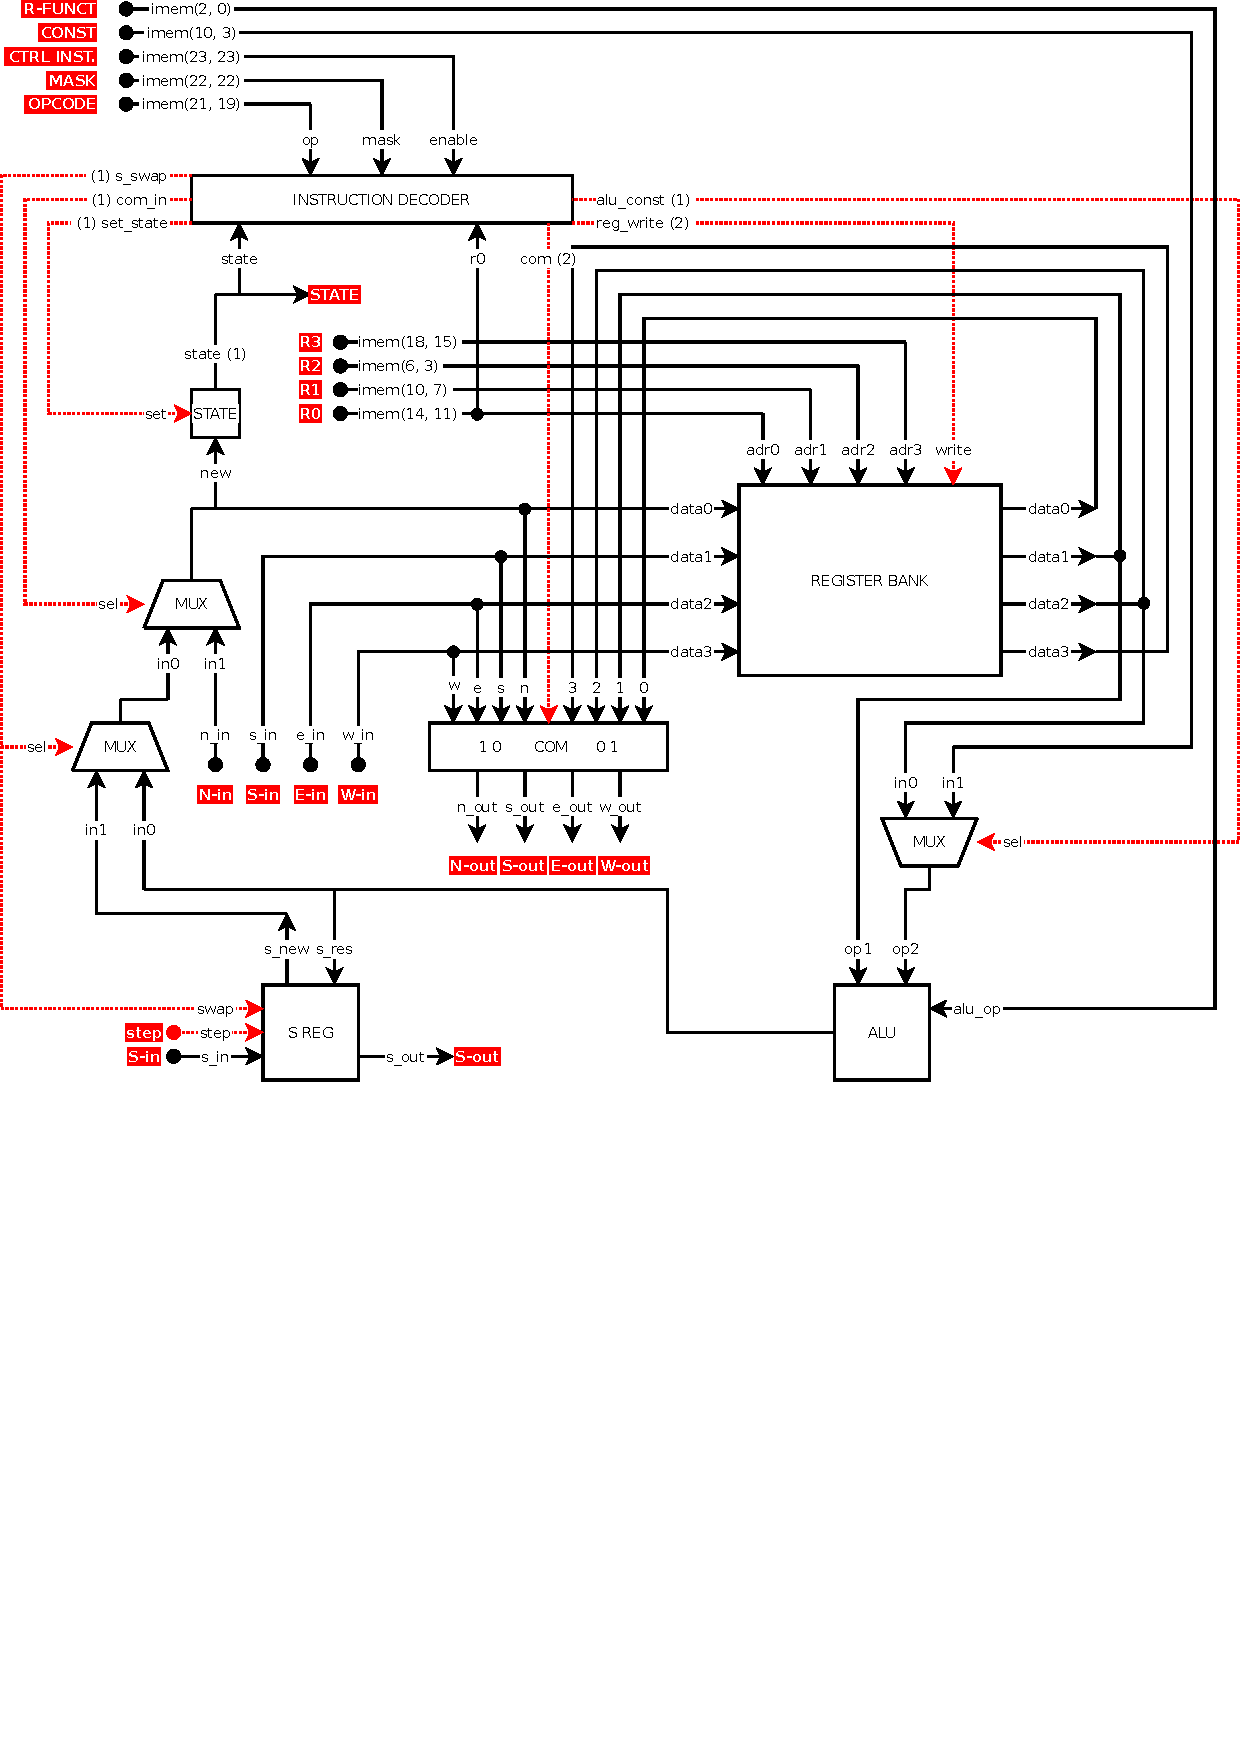
\includegraphics[width=\linewidth,clip,trim=0 0 0 0]
                  {fig/fpga/fpga-simd-arch.pdf}
  \caption{LENA SIMD architecture}
  \label{fig:fpga-simd-arch}
\end{figure}


\subsection{Components}
In this section we briefly describe the different components, their purpose, and
how they together form the data-path for the node. All components has been thoroughly
thought out and design to suit the \ac{SIMD} nodes.  

\subsubsection{Instruction Decoder}
Whenever a new instruction is received by the \ac{SIMD} node it is immediately 
decoded by the instruction decoder. Based on the enable-bit, mask-bit and OP-code
of the instruction correct control signals are set up for the remaining components
throughout the node.

For a list of all \ac{SIMD} instructions, see Appendix \ref{apx:simd-instruction-set}.

\subsubsection{Communication}
The communication component controls outbound data to adjacent \ac{SIMD} nodes in 
the grid array; north, south, east and west. The communication component is fairly 
simple and can either send register data or forward inbound data according to the 
counterclockwise forwarding scheme described in \ref{sec:simd-com}.

\subsubsection{Register Bank}
Each \ac{SIMD} node is equipped with $2^4 = 16$ 8-bit general purpose registers, 14 of
which are available for general storage during execution. The remaining 2 are
reserved for the special purpose registers {\tt \$zero} and {\tt \$state}.

\begin{table}[h]
  \centering
  \begin{tabularx}{\linewidth}{XXXXXXXXX}\toprule
    R0 & R1 & R2 & R3 & R4 & R5 & R6 & R7 \\ \midrule
    \tt \$zero & \tt \$r1 & \tt \$r2 & \tt \$r3 & \tt \$r4 & \tt \$r5 &
    \tt \$r6 & \tt \$r7\\ \bottomrule
  \end{tabularx}
  \begin{tabularx}{\linewidth}{XXXXXXXX}
    R8 & R9 & R10 & R11 & R12 & R13 & R14 & R15 \\ \midrule
    \tt \$r8 & \tt \$r9 & \tt \$r10 & \tt \$r11 & \tt \$r12 & \tt \$r13 &
    \tt \$r14 & \tt \$state\\ \bottomrule
  \end{tabularx}
  \caption{Registers in the SIMD nodes}
  \label{tab:simd-registers}
\end{table}


The register bank has been specially designed to suit the four-way data transfer by
allowing 4 registers to be read, or written, at during one clock-cycle.

\subsubsection{ALU}
Each \ac{SIMD} node has an 8-bit simple ALU supporting 8 arithmetic instructions: 
addition ({\sc add}), subtraction ({\sc sub}), set less than ({\sc slt}), {\sc and}, 
{\sc or}, equality check ({\sc eq}), shift logical left ({\sc sll}) and shift logical 
right ({\sc slr}). 

The main reason for only implementing the most basic arithmetic instruction was to save
space in the instruction set since addition, subtract, equality and less then are 
supported by special hardware inside the FPGA. All \ac{SIMD} node instructions carries
a 3-bit \ac{ALU} function at the end.

Upon researching image processing algorithms well suited for parallel processing, we
found that most of then could be implemented using only these 8 \ac{ALU} operations. 
Image processing algorithms such as median filter, various blur filters, edge detection, 
color manipulation such as inversion and thresholding are fully feasible using. More high
level arithmetic, such as multiply and divide by constants, can be implemented
through a series of additions, subtractions and shifts.

\CHECK{Proof-read this section!}
\CHECK{Add some reffernces?}
\CHECK{Talk about general programability?}

\subsubsection{Source Data Register}
The source data register, or just \ac{S-REG} for short, is a special purpose
register within the \ac{SIMD} node. It is a communication unit, separated form
the rest of the node so it can transfer new and processed image data through the
array while the \ac{SIMD} node is otherwise busy executing instructions.

\begin{figure}[h]
  \centering
  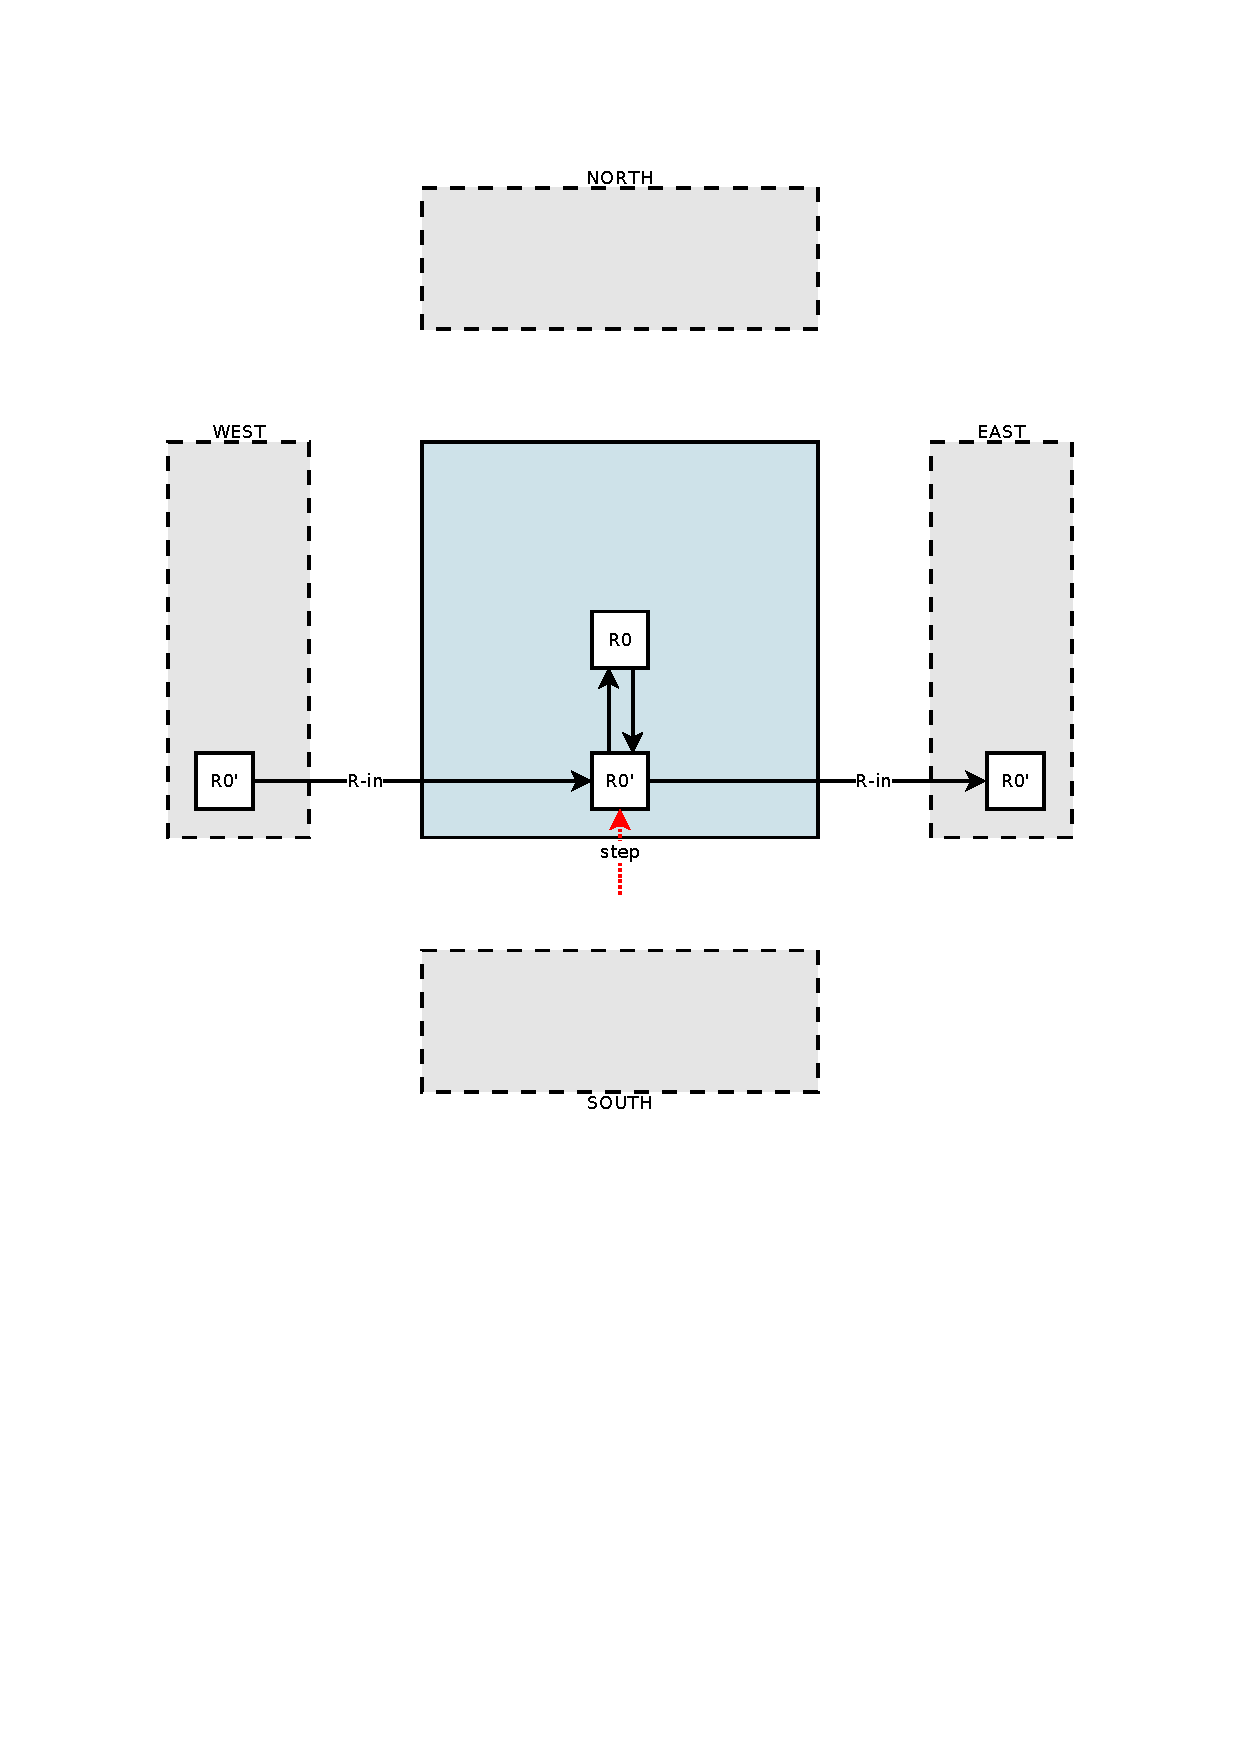
\includegraphics[width=\linewidth,clip,trim=0 0 0 0]
                  {fig/fpga/fpga-simd-s-reg.pdf}
  \caption[Source Data Flow.]{Source data flow through the \ac{LENA} \ac{SIMD} array.}
  \label{fig:fpga-simd-s-reg}
\end{figure}
 

The \ac{S-REG} is partly controlled by the \ac{SIMD} node instruction set where it
can swap data in and out from the \ac{S-REG} and partly by a special {\tt step} signal
sent from the \ac{DMA}.

\subsubsection{State Register}
In order to handle branches, through masked instructions, each \ac{SIMD} must have an
internal state register. Even though the register is 8-bit wide only the least 
significant bit is the current state for the node.

The state register can be written and read as any other register in the register
bank and the state can hence be shifted left or right in order to achieve nested
branches.

\subsection{Communication}\label{sec:simd-com}

Data exchange between \ac{SIMD} nodes are multiplexed in all directions. \ac{SIMD} nodes
are capable of sending source data in all directions during one clock cycle and storing
them within the next as shown in Figure \ref{fig:fpga-simd-send}.

\begin{figure}[h]
  \centering
  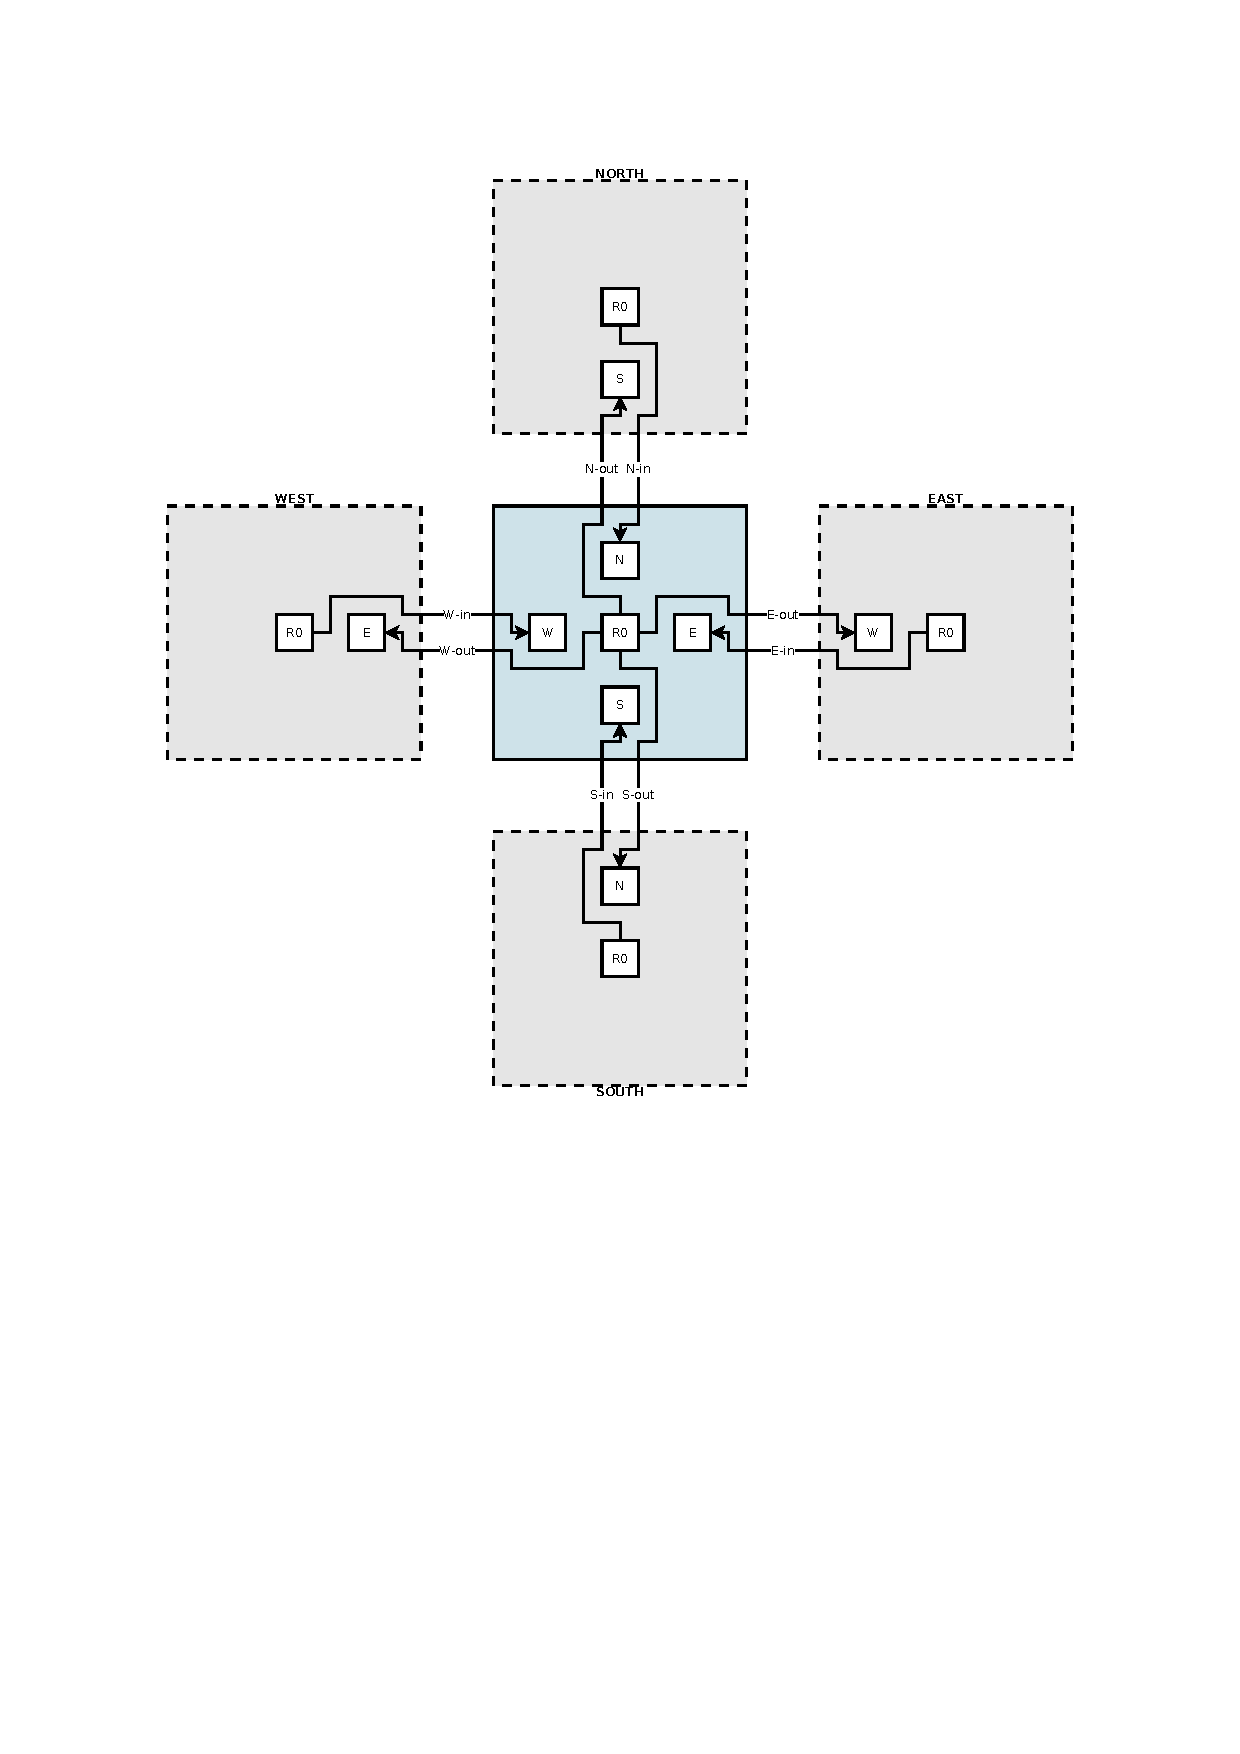
\includegraphics[width=\linewidth,clip,trim=0 0 0 0]
                  {fig/fpga/fpga-simd-send}
  \caption[Sending data]{Sending and recieving data from and to adjacent nodes in the \ac{LENA} \ac{SIMD} array.}
  \label{fig:fpga-simd-send}
\end{figure}


\subsubsection{Forwarding}
The counterclockwise forwarding, illustrated by Figure \ref{fig:fpga-simd-fwrd}, is an 
optimized way we devised for distributing a 3$\times$3 array of source data to all 
\ac{SIMD} nodes in the \ac{SIMD} array using only 3 clock cycles; send, forward and sore, 
and store.

\begin{figure}[h]
  \centering
  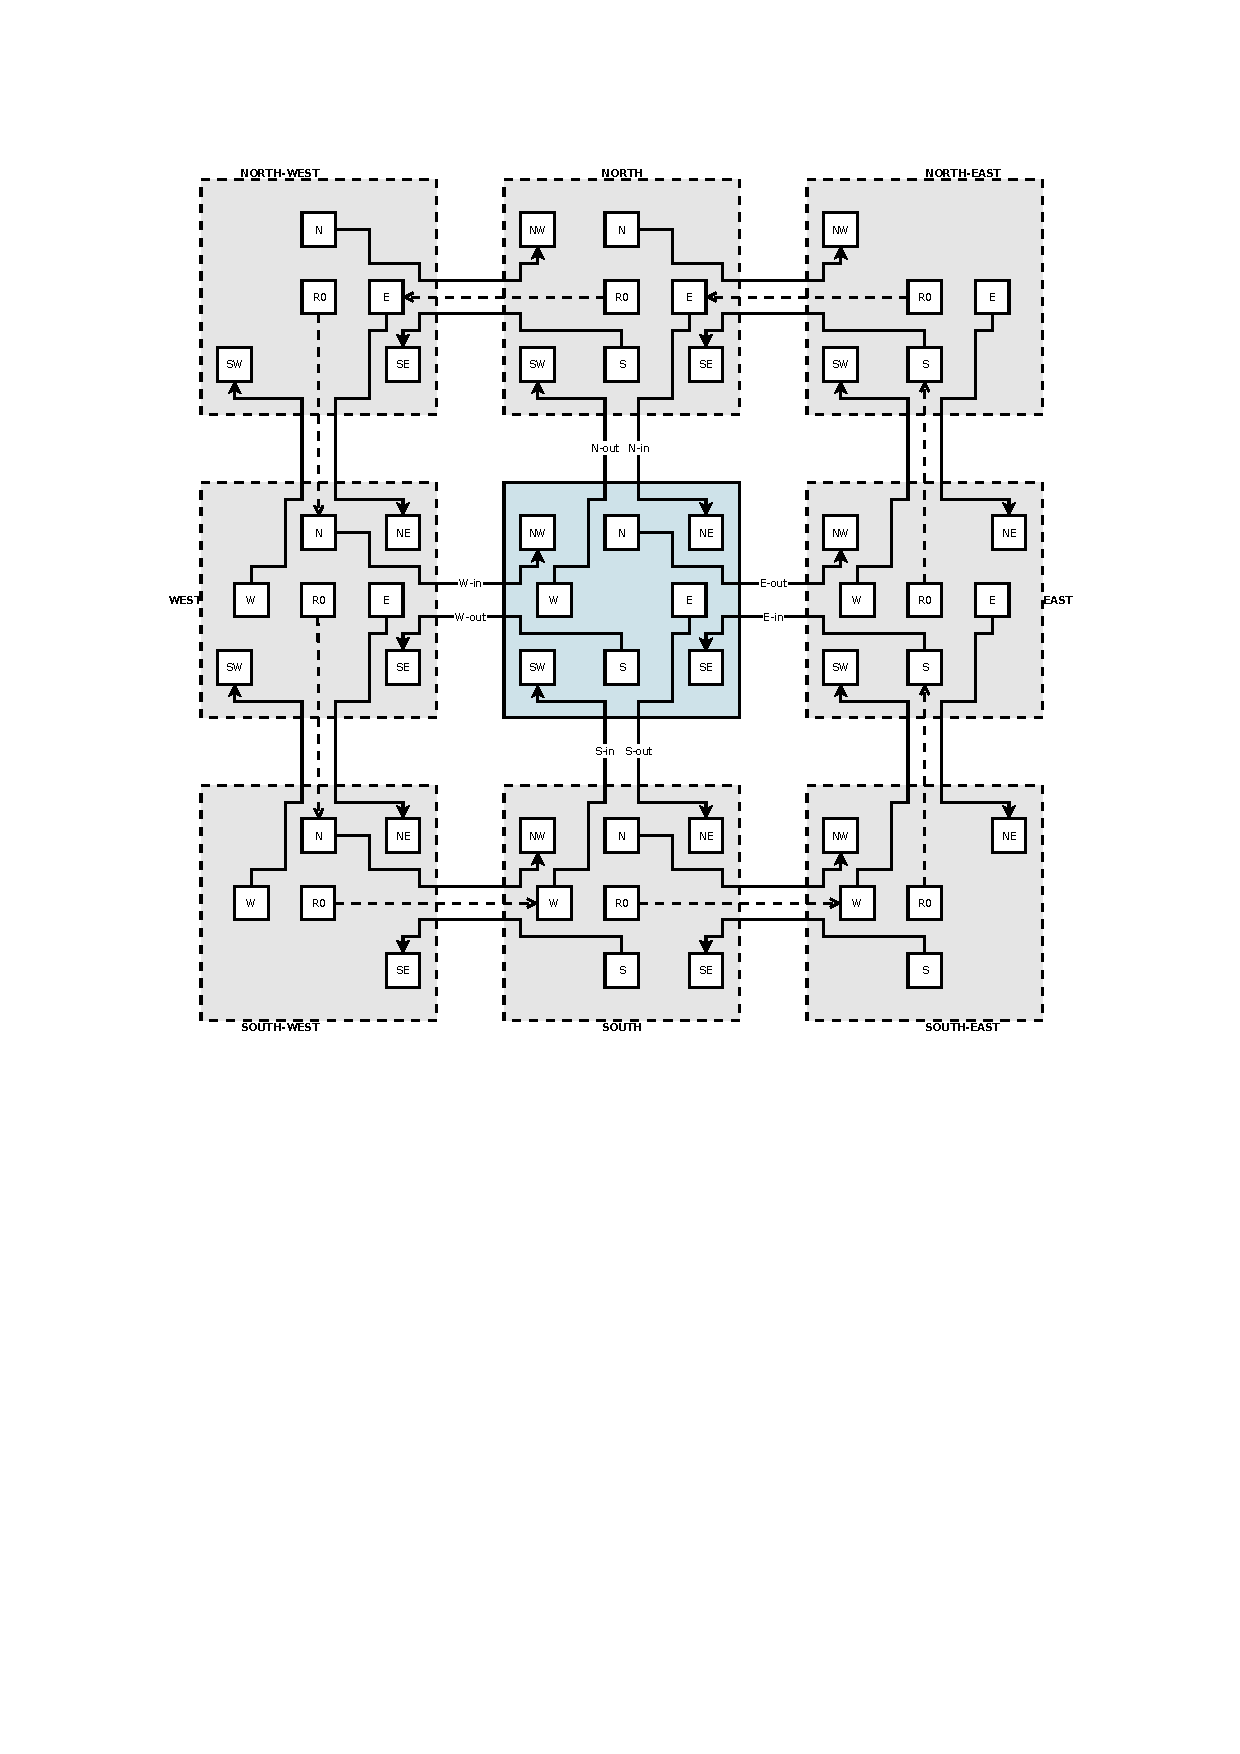
\includegraphics[width=\linewidth,clip,trim=0 0 0 0]
                  {fig/fpga/fpga-simd-fwrd.pdf}
  \caption[Data forwarding.]{Counterclockwise forwarding for nonadjacent nodes in the \ac{LENA} \ac{SIMD} array.}
  \label{fig:fpga-simd-fwrd}
\end{figure}


\TODO{We invented this one by ourselves! Should we brag some more?}

\subsection{Instruction Set}
The \ac{SIMD} node instruction set, detailed in Appendix \ref{apx:simd-instruction-set}, 
controls all aspects of the \ac{SIMD} node. It has been designed with regularity in mind 
in order to keep the number of special cases in the hardware to a minimum with as few 
formats as possible.

Much of the design behind the instruction set is borrowed from \ac{MIPS} which also 
favors regularity in order to simplify the hardware, thus enhancing the performance.

\subsubsection{Branching}
Since all nodes run the same instructions, both parts of a branch must be
executed. Nodes are setting the {\tt state} to 1 in order to indicate that they
are executing within that part of the branch. An example of single branching is
shown in Listing \ref{lst:single-branch}.

{\sc \color{green} LENA-assembly here (fixed)}

Since the state register is 8 bits, it is possible to have up to 8 nested
branches by shifting the current state left and adding the new state to the
end. Listing \ref{lst:multibranch} contains code which performs such a
multilevel branch.

{\sc \color{green} LENA-assembly here (fixed)}
